\documentclass{article}
\usepackage{titlesec}
\usepackage{graphicx}
\usepackage{authblk}
\usepackage{listings}
\usepackage{xcolor}
\usepackage{amsmath}
\usepackage{algorithm}
\usepackage[noend]{algpseudocode}
\usepackage[a4paper,
            bindingoffset=0.2in,
            left=0.5in,
            right=0.5in,
            top=0.75in,
            bottom=0.75in,
            footskip=.25in]{geometry}

\definecolor{mGreen}{rgb}{0,0.6,0}
\definecolor{mGray}{rgb}{0.5,0.5,0.5}
\definecolor{mPurple}{rgb}{0.58,0,0.82}
\definecolor{backgroundColour}{rgb}{0.95,0.95,0.92}

\lstdefinestyle{CStyle}{
    backgroundcolor=\color{backgroundColour},   
    commentstyle=\color{mGreen},
    keywordstyle=\color{magenta},
    numberstyle=\tiny\color{mGray},
    stringstyle=\color{mPurple},
    basicstyle=\footnotesize,
    breakatwhitespace=false,         
    breaklines=true,                 
    captionpos=b,                    
    keepspaces=true,                 
    numbers=left,                    
    numbersep=5pt,                  
    showspaces=false,                
    showstringspaces=false,
    showtabs=false,                  
    tabsize=2,
    language=C
}

\titlespacing*{\section}
{0pt}{5.5ex plus 1ex minus .2ex}{4.3ex plus .2ex}
\titlespacing*{\subsection}
{0pt}{5.5ex plus 1ex minus .2ex}{4.3ex plus .2ex}

\makeatletter
\def\BState{\State\hskip-\ALG@thistlm}
\makeatother

\title{Lab \#1a}
\author{Cody Raposa}
\affil{ELEC2850 Microcontrollers Using C Programming}

\begin{document}
\maketitle
\begin{flushleft}
  \section{Problem Statement}
  Create a program that will calculate the area of any tringle with sides \textit{a}, \textit{b}, and \textit{c}. The program will then output the area of the triangle, using Heron's formula. If the area is negative it will prompt the user that the triangle cannot exist.
  %\section{Assumptions}
  %\section{Pseudocode}
  \section{Algorithm}
  \begin{algorithm}
    \caption{Triangle Calculation}\label{euclid}
    \begin{algorithmic}[1]
      %\Procedure{MyProcedure}{}
      \State $a \gets$ input from user for side a
      \State $b \gets$ input from user for side b
      \State $c \gets$ input from user for side c
      \State $s \gets \frac{a+b+c}{2}$
      \State $area \gets \sqrt{s(s-a)(s-b)(s-c)}$
      \If {$s < $} 0 \Return Not a triangle
      \EndIf
      \State \Return $area$
      %\EndProcedure
    \end{algorithmic}
  \end{algorithm}
  \newpage
  \section{Flowchart}
  \begin{figure}[!ht]
    \centering
    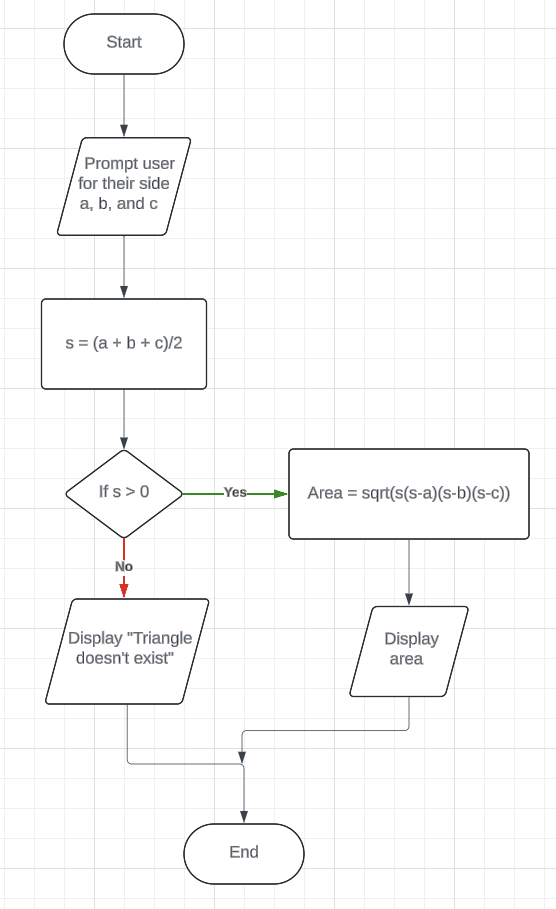
\includegraphics[scale=0.95]{Flowchart.png}
    \caption{Flowchart for the program.}
  \end{figure}
  \newpage
  \section{Part 2}
  \subsection{Question 1}
  The code does not not include the library stdio.h, vscode and GCC will fix in the precompile stage, however adding stdio.h will fix the issue.
  \begin{figure}[!ht]
    \centering
    \lstinputlisting[style=CStyle]{Lab1a_P2_Q1.c}
    \caption{The code for question 1.}
  \end{figure}
  \begin{figure}[!ht]
    \centering
    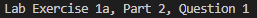
\includegraphics[width=\linewidth]{Q1-output.png}
    \caption{Output of Q1.}
  \end{figure}
  \subsection{Question 2}
  \begin{figure}[!ht]
    \centering
    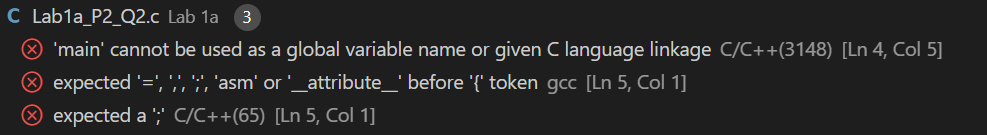
\includegraphics[width=\linewidth]{Q2-error.png}
    \caption{Error message with VSCode error lens Q2.c}
  \end{figure}
  Fixing this problem requires only adding () after main. This will allow the code to compile as C recognizes it as a function now.
  \begin{figure}[!ht]
    \centering
    \lstinputlisting[style=CStyle]{Lab1a_P2_Q2.c}
    \caption{The code for question 2.}
  \end{figure}
  \begin{figure}[!ht]
    \centering
    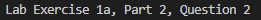
\includegraphics[width=\linewidth]{Q2-output.png}
    \caption{Output of Q2.}
  \end{figure}
  \subsection{Question 3}
  There was no error in Q3 however because our main function is an int, it must return 0 to safely exit the program.
  \begin{figure}[!ht]
    \centering
    \lstinputlisting[style=CStyle]{Lab1a_P2_Q3.c}
    \caption{The code for question 3.}
  \end{figure}
  \begin{figure}[!ht]
    \centering
    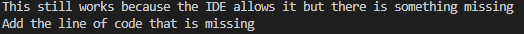
\includegraphics[width=\linewidth]{Q3-output.png}
    \caption{Output of Q3.}
  \end{figure}
  \subsection{Question 4}
  \begin{figure}[!ht]
    \centering
    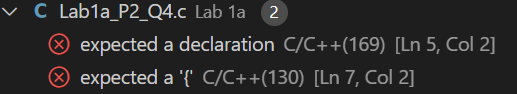
\includegraphics[width=\linewidth]{Q4-error.png}
    \caption{Error message with VSCode error lens Q4.c}
  \end{figure}
  Fixing this error requires adding a \{ to the begining of the main function. This is because C doesn't understand where the function starts.
  \begin{figure}[!ht]
    \centering
    \lstinputlisting[style=CStyle]{Lab1a_P2_Q4.c}
    \caption{The code for question 4.}
  \end{figure}
  \begin{figure}[!ht]
    \centering
    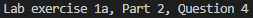
\includegraphics[width=\linewidth]{Q4-output.png}
    \caption{Output of Q4.}
  \end{figure}
  \subsection{Question 5}
  \begin{figure}[!ht]
    \centering
    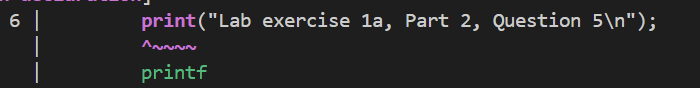
\includegraphics[width=\linewidth]{Q5-error.png}
    \caption{Error message when compiling Q5.c}
  \end{figure}
  The function print() does not exist and is instead printf. Changing this will allow the code to compile.
  \begin{figure}[!ht]
    \centering
    \lstinputlisting[style=CStyle]{Lab1a_P2_Q5.c}
    \caption{The code for question 5.}
  \end{figure}
  \begin{figure}[!ht]
    \centering
    
\includegraphics[width=\linewidth]{Q5-output.png}
    \caption{Output of Q5.}
  \end{figure}
  \subsection{Question 6}
  \begin{figure}[!ht]
    \centering
    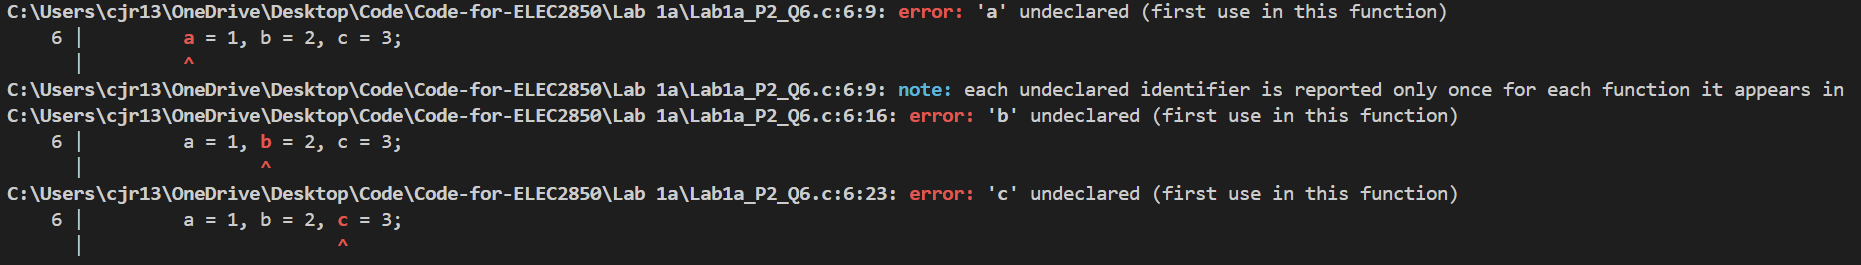
\includegraphics[width=\linewidth]{Q6-error.png}
    \caption{Error message when compiling Q6.c}
  \end{figure}
  The variables a, b, and c have not been delcared so C hasn't allocated memory for them. Adding int or float infront of them will fix this issue.
  \begin{figure}[!ht]
    \centering
    \lstinputlisting[style=CStyle]{Lab1a_P2_Q6.c}
    \caption{The code for question 6.}
  \end{figure}
  \begin{figure}[!ht]
    \centering
    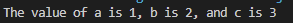
\includegraphics[width=\linewidth]{Q6-output.png}
    \caption{Output of Q6.}
  \end{figure}
  \subsection{Question 7}
  \begin{figure}[!ht]
    \centering
    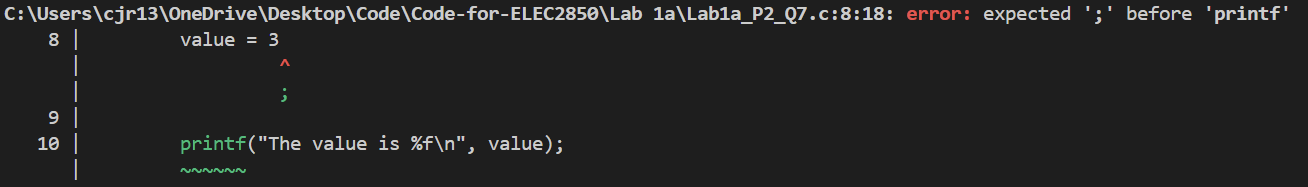
\includegraphics[width=\linewidth]{Q7-error.png}
    \caption{Error message when compiling Q7.c}
  \end{figure}
  Line 8 wasn't properly ended with a ;. Adding this will fix the issue, and stop C from reading the line as (value=3printf...)
  \begin{figure}[!ht]
    \centering
    \lstinputlisting[style=CStyle]{Lab1a_P2_Q7.c}
    \caption{The code for question 7.}
  \end{figure}
  \begin{figure}[!ht]
    \centering
    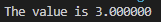
\includegraphics[width=\linewidth]{Q7-output.png}
    \caption{Output of Q7.}
  \end{figure}
  \subsection{Question 8}
  \begin{figure}[!ht]
    \centering
    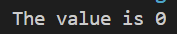
\includegraphics[width=\linewidth]{Q8-error.png}
    \caption{The output for Q8.}
  \end{figure}
  Because \%d is being used instead of \%f the output is 0 instead of 28.50. Changing \%d to \%f will fix this issue.
  \begin{figure}[!ht]
    \centering
    \lstinputlisting[style=CStyle]{Lab1a_P2_Q8.c}
    \caption{The code for question 8.}
  \end{figure}
  \begin{figure}[!ht]
    \centering
    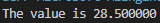
\includegraphics[width=\linewidth]{Q8-output.png}
    \caption{Output of Q8.}
  \end{figure}
  \newpage
  \subsection{Question 9}
  \begin{figure}[!ht]
    \centering
    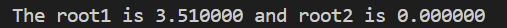
\includegraphics[width=\linewidth]{Q9-error.png}
    \caption{The output for Q9.}
  \end{figure}
  The output for root2 is 0 becuase the variable for root2 in not included in the printf statement. Adding root2 after root1 to the printf statement will fix this issue.
  \begin{figure}[!ht]
    \centering
    \lstinputlisting[style=CStyle]{Lab1a_P2_Q9.c}
    \caption{The code for question 9.}
  \end{figure}
  \begin{figure}[!ht]
    \centering
    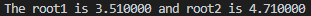
\includegraphics[width=\linewidth]{Q9-output.png}
    \caption{Output of Q9.}
  \end{figure}
  \newpage
  \section{Part 3}
  \begin{figure}[!ht]
    \centering
    \lstinputlisting[style=CStyle]{Lab1a_P3.c}
    \caption{The code for Part 3.}
  \end{figure}
  \begin{figure}[!ht]
    \centering
    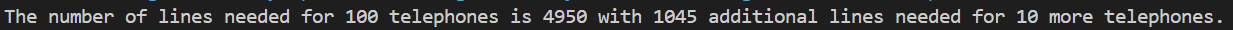
\includegraphics[width=\linewidth]{P3-Output.png}
    \caption{The output for Part 3.}
  \end{figure}
\end{flushleft}
\end{document}